\documentclass{article}
\setlength{\parskip}{5pt} % esp. entre párrafos
\setlength{\parindent}{0pt} % esp. al inicio de un párrafo
\usepackage{amsmath} % mates
\usepackage[sort&compress,numbers]{natbib} % referencias
\usepackage{url} % que las URLs se vean lindos
\usepackage[top=25mm,left=20mm,right=20mm,bottom=25mm]{geometry} % márgenes
\usepackage{hyperref} % ligas de URLs
\usepackage{graphicx} % poner figuras
\usepackage[spanish]{babel} % otros idiomas

\author{Raul L.} % author
\title{Pr\'{a}ctica 3:  Teoría de colas} %título
\date{\today}

\begin{document} % inicia contenido

\maketitle % cabecera


\section{Introducci\'{o}n}\label{intro} % sección y etiqueta



La teoría de colas es un área de las matemáticas que estudia el comportamiento de líneas de espera. Los trabajos que están esperando ejecución en un cluster esencialmente forman una línea de espera. Medidas de interés que ayudan caracterizar el comportamiento de una línea de espera incluye, el tiempo total de ejecución. En esta práctica se estudiará el efecto del orden de ejecución de trabajos y el número de núcleos utilizados en esta medida\citep{ejemplo}.

\section{Objetivo}
Examinar las diferencias en los tiempos de ejecución variando algunos o todos de los siguientes aspectos:

El orden de los números.

La cantidad de núcleos asignados al cluster.

La variante de la rutina para determinar si un número es primo\\
Aplicando pruebas estadísticas adecuadas y visualización científica clara e informativa.
\citep{ejemplo}.


\section{C\'{o}digo}
Con el siguiente código se examinó como las diferencias en los tiempos de ejecución de los diferentes ordenamientos cambian cuando se varía el número de núcleos asignados al clúster, utilizando como datos de entrada diferentes procesos para obtener primos grandes. Además el programa hace un análisis estadístico para determinar si tienen una relación significativa o no, asímismo, este se graficó en barras horizontales .\\
El c\'{o}digo base se sac\'{o} del repositorio de Elisa Schaeffer.

\\ Código en Phyton 

\\\url{https://github.com/satuelisa/Simulation/blob/master/QueuingTheory/fixedshuffle.py}\\


**Código creado en Python**\\

\url{https://github.com/Raullr28/Resultados/tree/main/P3}

Iniciamos definiendo dos formas de encontrar números, teniendo el método para encontrar números primos se establecen los 3 parámetros de recorrido, las repeticiones y los núcleos presentes.
\begin{figure}[h]
     \centering
     \includegraphics[width=70mm]{imagenes/primos.png}
        \caption{Recorte del código de Raul L. del código de Python 
    \url{https://github.com/Raullr28/Resultados/tree/main/P3}}
     \label{}
 \end{figure}
 \newpage
 Continuamos con un ciclo donde entran en juego los parámetros anteriormente dados, se hace un recorrido con el primer método para encontrar números primos utilizando los 3 parámetros de recorrido, al igual que con el segundo método para encontrar números primos lo cual genera un ciclo completo.
 El ciclo se repite dependiendo el numero de núcleos de cada computadora.
 \begin{figure}[h]
     \centering
     \includegraphics[width=70mm]{imagenes/ciclo.png}
        \caption{Recorte del código de Raul L. del código de Python 
    \url{https://github.com/Raullr28/Resultados/tree/main/P3}}
     \label{}
 \end{figure}
\newpage
Se utilizó un sistema estadístico para relacionar si existía un una dependencia entre los valores dados en el ciclo. 
\begin{figure}[h]
     \centering
     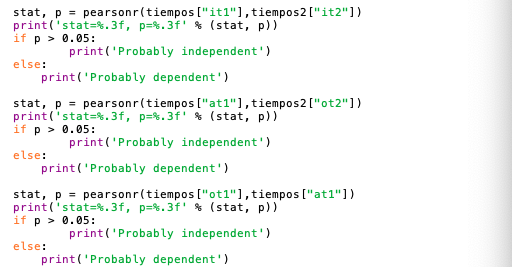
\includegraphics[width=70mm]{imagenes/Captura de Pantalla 2022-03-01 a la(s) 15.37.37.png}
        \caption{Recorte del código de Raul L. del código de Python 
    \url{https://github.com/Raullr28/Resultados/tree/main/P3}}
     \label{}
 \end{figure}
 
 
% Computational Results
\section{Resultados}
En la figura se muestra el tiempo que transcurrió el código al procesar las diferentes formas en encontrar los números primos, para ello, se varió el número de núcleos.


 \begin{figure}[h]
     \centering
     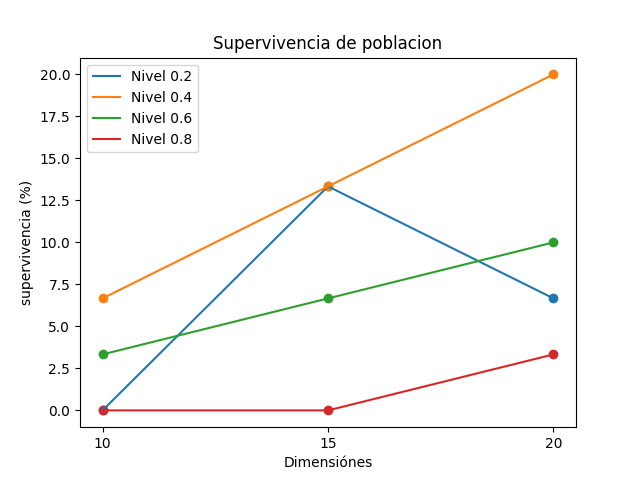
\includegraphics[width=100mm]{imagenes/Figure_1.png}
        \caption{Gráfica tomada del repositorio de Raul L. del código de Python 
    \url{https://github.com/Raullr28/Resultados/blob/main/P3/Figure_1.png}}
     \label{}
 \end{figure}
 

 \begin{figure}[h]
     \centering
     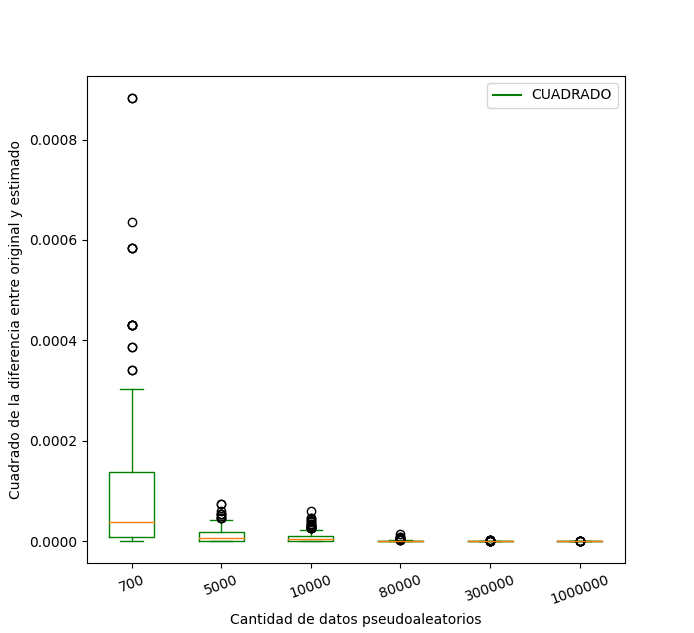
\includegraphics[width=100mm]{imagenes/Figure_2.png}
        \caption{Gráfica tomada del repositorio de Raul L. del código de Python 
    \url{https://github.com/Raullr28/Resultados/blob/main/P3/Figure_2.png}}
     \label{}
 \end{figure}
 
 
 \newpage
 

 \section{Conclusión}

 Se creó un código que puede variar el número de núcleos para la correcta realización de la práctica 3, así como también se analizaron diferentes formas de en encontrar los números primos, para ello, se midió el tiempo en cada procedimiento, utilizando un análisis estadístico, con el cual se obtuvo una relación entre los números de núcleos y el tiempo realizado por cada proceso, lo cual se puede observar en la gráfica de lineas.


 \bibliography{biblio.bib}
 \bibliographystyle{plainnat}

 \end{document}
